
\documentclass{standalone}
\usepackage[svgnames]{xcolor}
\usepackage{pgfplots}
\pgfplotsset{compat=newest}
\usepackage[sfdefault]{FiraSans}
\usepackage{FiraMono}
\renewcommand*\familydefault{\sfdefault}
\begin{document}
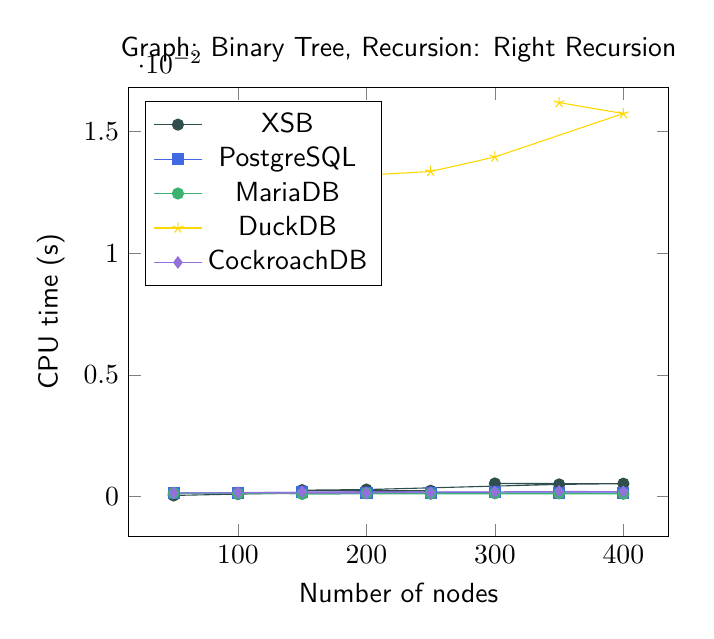
\begin{tikzpicture}
    \begin{axis}[
        title={Graph: Binary Tree, Recursion: Right Recursion},
        xlabel={Number of nodes},
        ylabel={CPU time (s)},
        legend pos={north west},
        ymax=0.01679314999999998
    ]
    \addplot+[DarkSlateGray, mark options={color=DarkSlateGray}] coordinates {(50,4.9000000000000446e-05) (100,0.000103999999999998) (250,0.0002404999999999975) (150,0.000264500000000001) (200,0.0002909999999999995) (350,0.0005025000000000029) (400,0.000532500000000005) (300,0.0005414999999999964)};
\addlegendentry{XSB}
\addplot+[RoyalBlue, mark options={color=RoyalBlue}] coordinates {(250,0.00013245000000000617) (200,0.00013545000000000917) (350,0.00013944999999998542) (50,0.0001487000000000016) (400,0.00015409999999999036) (100,0.00015944999999997767) (150,0.00017854999999999954) (300,0.00018740000000000423)};
\addlegendentry{PostgreSQL}
\addplot+[MediumSeaGreen, mark options={color=MediumSeaGreen}] coordinates {(150,0.00010910000000000086) (400,0.00011735000000001605) (250,0.00011764999999996917) (100,0.0001213499999999923) (350,0.00013355000000001005) (300,0.00013445000000000817) (200,0.00014005000000000267) (50,0.00014279999999999848)};
\addlegendentry{MariaDB}
\addplot+[Gold, mark options={color=Gold}] coordinates {(200,0.008898850000000014) (50,0.00969790000000001) (150,0.012395750000000011) (100,0.012920750000000009) (250,0.013357950000000007) (300,0.013954099999999997) (400,0.01573795) (350,0.01618750000000002)};
\addlegendentry{DuckDB}
\addplot+[MediumPurple, mark options={color=MediumPurple}] coordinates {(200,0.0001466999999999996) (50,0.00015565000000000717) (250,0.0001635500000000123) (100,0.0001669500000000268) (300,0.0001914499999999819) (150,0.00019314999999997529) (400,0.00020105000000003592) (350,0.00021444999999997716)};
\addlegendentry{CockroachDB}

    \end{axis}
\end{tikzpicture}
\end{document}
